
\chapter{发光二极管}
\label{chap:introduction}

发光二极管也是由一个PN结构成,具有单向导电性。但其正向工作电压(开启电压)比普通二极管高,约为1~2.5V,反向击穿电压比普通二极管低,约5V左右。当正向电流达到1mA左右时开始发光,发光强度近似与工作电流成正比;但工作电流达到一定数值时,发光强度逐渐趋于饱和,与工作电流成非线性关系。一般小型发光二极管正向工作电流为10~20mA,最大正向工作电流为30~50mA。

发光二极管的外形可以做成矩形、圆形、字形、符号形等多种形状,又有红、绿、黄、橙、红外等多种颜色。它具有体积小、功耗低、容易驱动、光效高、发光均匀稳定、响应速度快以及寿命长等特点。

\begin{figure}[!htbp]
    \centering
    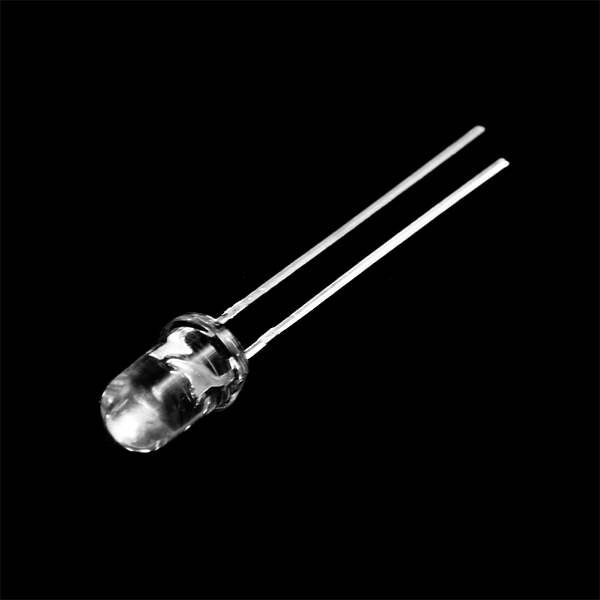
\includegraphics[width=0.45\textwidth]{08285-01}
    \caption{LED - Super Bright Green}
    \label{fig:08285-01}
\end{figure}

\section{典型电路}
LED电路是由电源,电阻,发光二极管串联组成的, 如图~\ref{fig:led_circuit}

\begin{figure}[H]
    \centering
    % 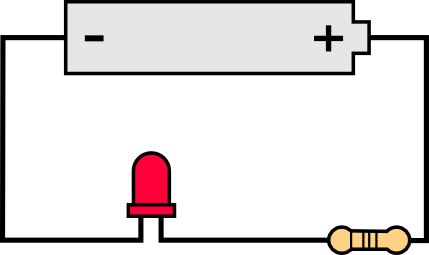
\includegraphics[width=0.8\textwidth]{led_circuit}
    \begin{circuitikz}
      \draw[color=black, thick, scale=2]
      (0,0)
      to[R=$R_1$] (2,0)
      to[empty led](4,0)
      to[short] (4,0) -- (4,2)
      to[battery1] (0,2)
      to[short] (0,2) -- (0,0)
      ;
    \end{circuitikz}
    \caption{LED Circuit}
    \label{fig:led_circuit}
\end{figure}


\section{电阻计算}

下图来自深圳市昱申科技有限公司的LED模块\href{https://www.sparkfun.com/datasheets/Components/YSL-R542G5C-A14.pdf}{YSL-R542G5C-A14}

\begin{figure}[H]
    \centering
    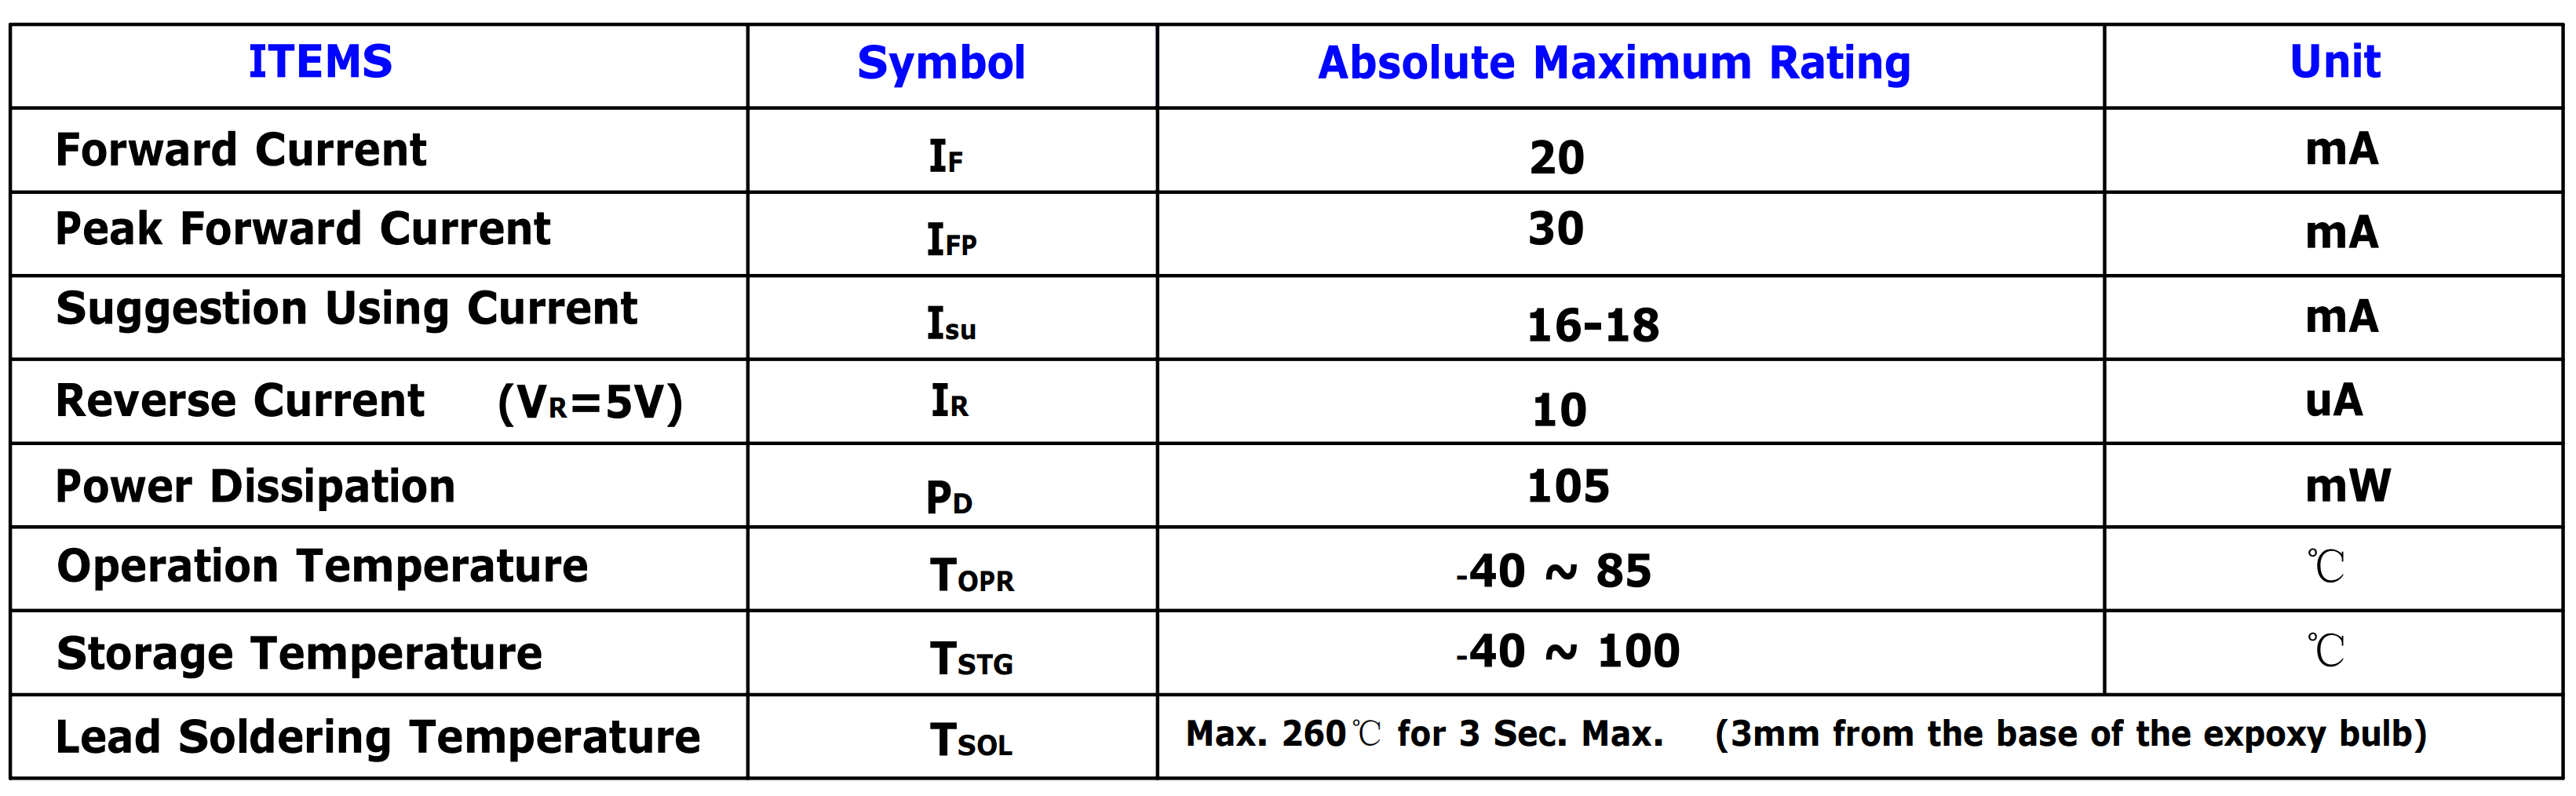
\includegraphics[width=0.8\textwidth]{led_current}
    \caption{LED Current}
    \label{fig:led_current}
\end{figure}

\begin{figure}[H]
    \centering
    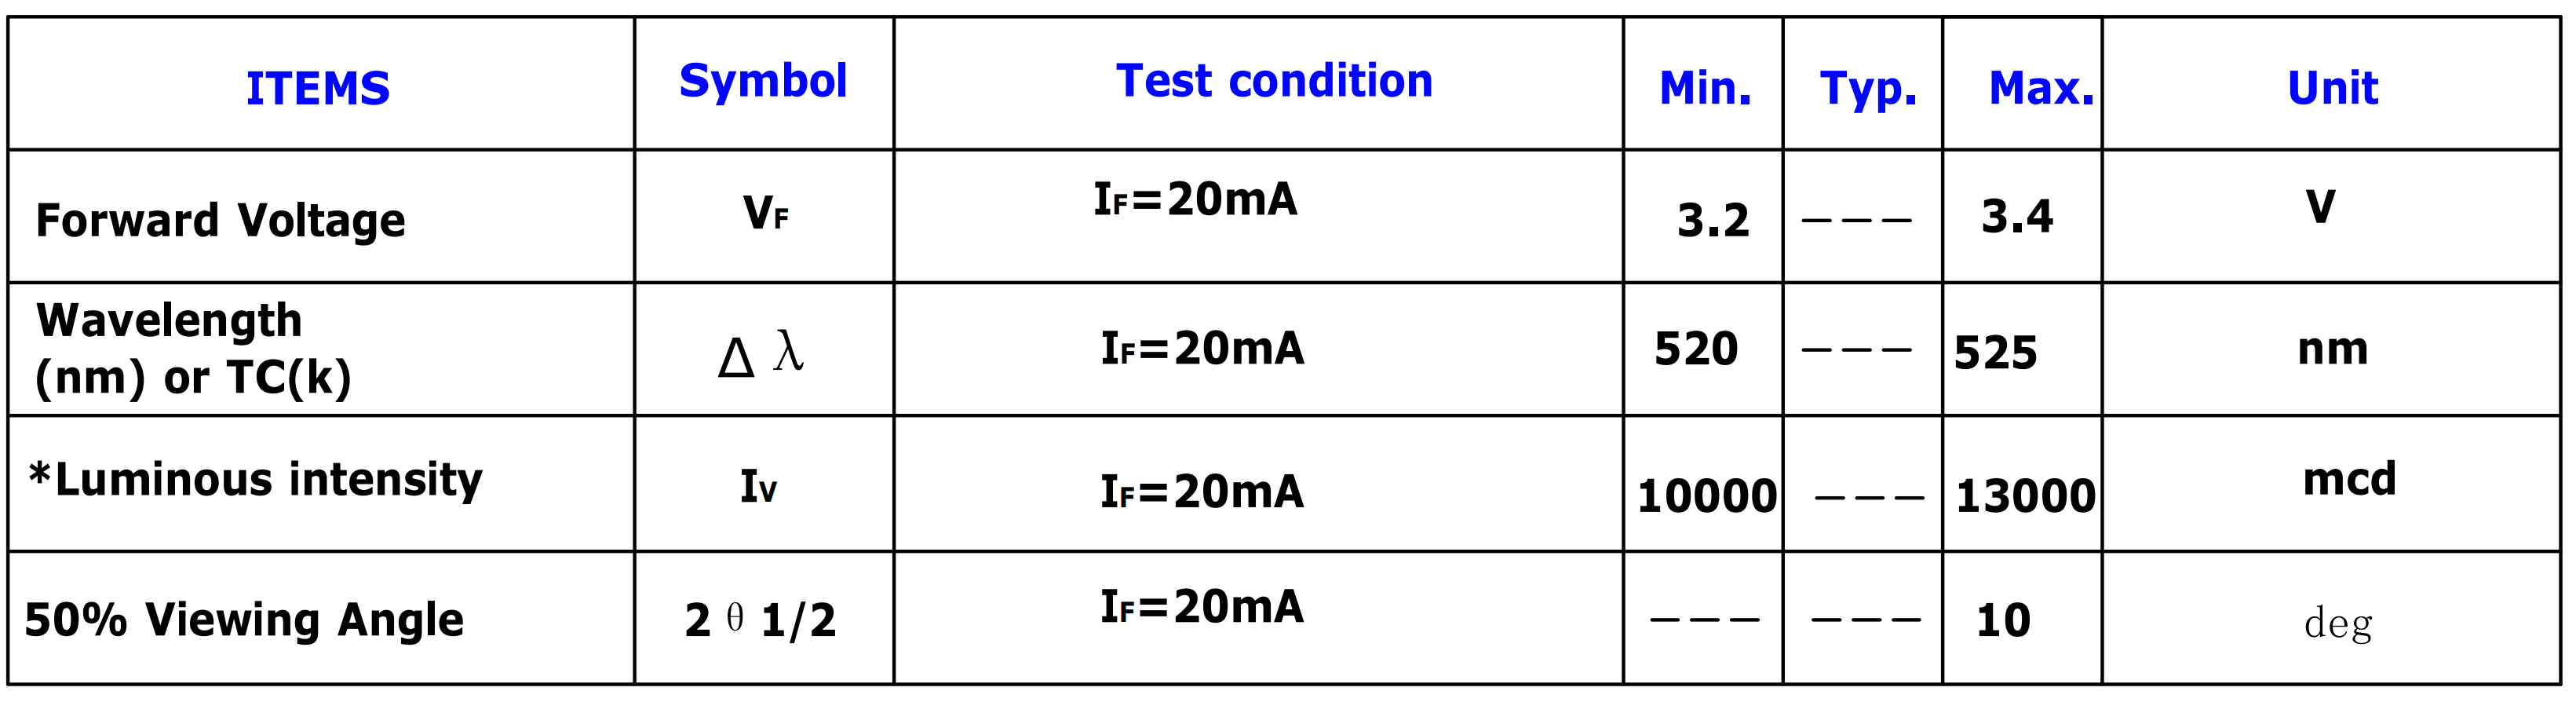
\includegraphics[width=0.8\textwidth]{led_voltage}
    \caption{LED Voltage}
    \label{fig:led_voltage}
\end{figure}

需要注意的是这几项Forward Current, Peak Forward Current, Suggestion Using Current和Forward Voltage,建议使用电流是$I_{su}$, $16mA \leq I_{su} \leq 18mA$, Forward Voltage $V_f \approx 3.3V$, $V_{cc}$应大于$V_f$ 这里选择$I_{su}=17mA, V_{cc}=5V$, 功耗$P=U*I_{su}$, 尽量使功耗最低。

\begin{equation}\label{eq:led_calc_r}
\begin{aligned}
        V_{cc} & = V_R + V_f \\
        R & = \frac{V_{cc} - V_f}{I_{su}} \\
        R & = \frac{5V - 3.3V}{17mA} \\
        R & = 100\Omega \\
        P & = V_{cc} * I_{su} \\
        P & = 5V * 17mA = 85mW
\end{aligned}
\end{equation}

LED说明 \\
\indent $\blacksquare$ LED导通才发光 \\
\indent $\blacksquare$ LED通过电流太大容易损坏(典型最大值20毫安) \\
\indent $\blacksquare$ LED反向电压过大容易损坏 \\


\begin{figure}[H]
    \centering
    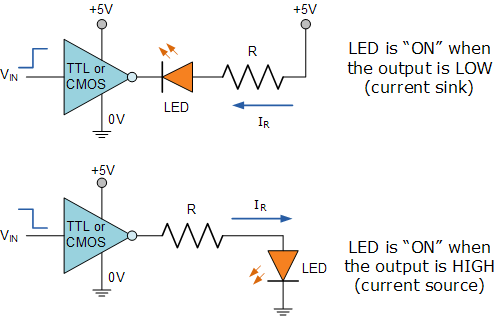
\includegraphics[width=0.8\textwidth]{ic_driver_circuit}
    \caption{IC Driver Circuit}
    \label{fig:ic_driver_circuit}
\end{figure}

\begin{figure}[H]
    \centering
    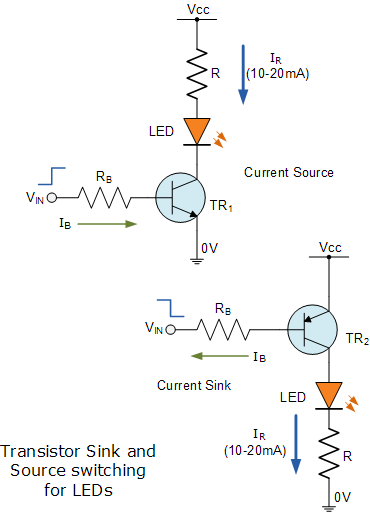
\includegraphics[width=0.8\textwidth]{transistor_driver_circuit}
    \caption{Transistor Driver Circuit}
    \label{fig:transistor_driver_circuit}
\end{figure}

\textbf{为什么电路要串联电阻?}

\textbf{为什么要选择$V_{cc}=5V$?}

\textbf{串联电阻的作用是什么?}
